\subsection{Ibrutinib (Ibr)}
Ibrutinib (Ibr) is a chemotherapic drug (Fig. \ref{fig:Ibr}) used as a deactivator of Bruton tyrosine kinase (BTK). Whenever B cells receptor signaling has an aberrhant behaviour alongside antigen-dependent activation BTK is involved, this also includes the pathogenesis of many lymphocytes-related malignancies \cite{ibr-1}.\\
Ibr blocks B cell antigen receptor signalling through an irreversible covalent bond with Cys-481 of BTK, hence reducing malignant B cell proliferation and inducing cell death.\\
The drug reaches its maximum concentration in plasma ($953\,\text{ng}\cdot\text{h}/\text{mL}$ at dosage of $560\,\text{mg}/\text{day}$) in 1-2 h and is widely distributed in the body. The major route of elimination is metabolism. It is metabolised by hepatic cytochrome P450 3A enzymes. It has an elimination half-life of 4-6 h via faeces.\\
It has been shown that Ibr has a high tolerance level in the body, clinical studies have shown that dose limiting events are not observed even with prolonged dosing \cite{ibr-2} but saturation of the active site of BTK was reached after a single dose of 2.5 to 20 mg/kg \cite{ibr-pubchem}. Reported dosages administered Ibr in 1.25, 2.5, 5.0, 8.3, 12.5, and 17.5 mg/kg/day for 28 day orally, with a 7-day rest period \cite{ibr-2}.
\begin{figure}[htbp!]
	\centering
	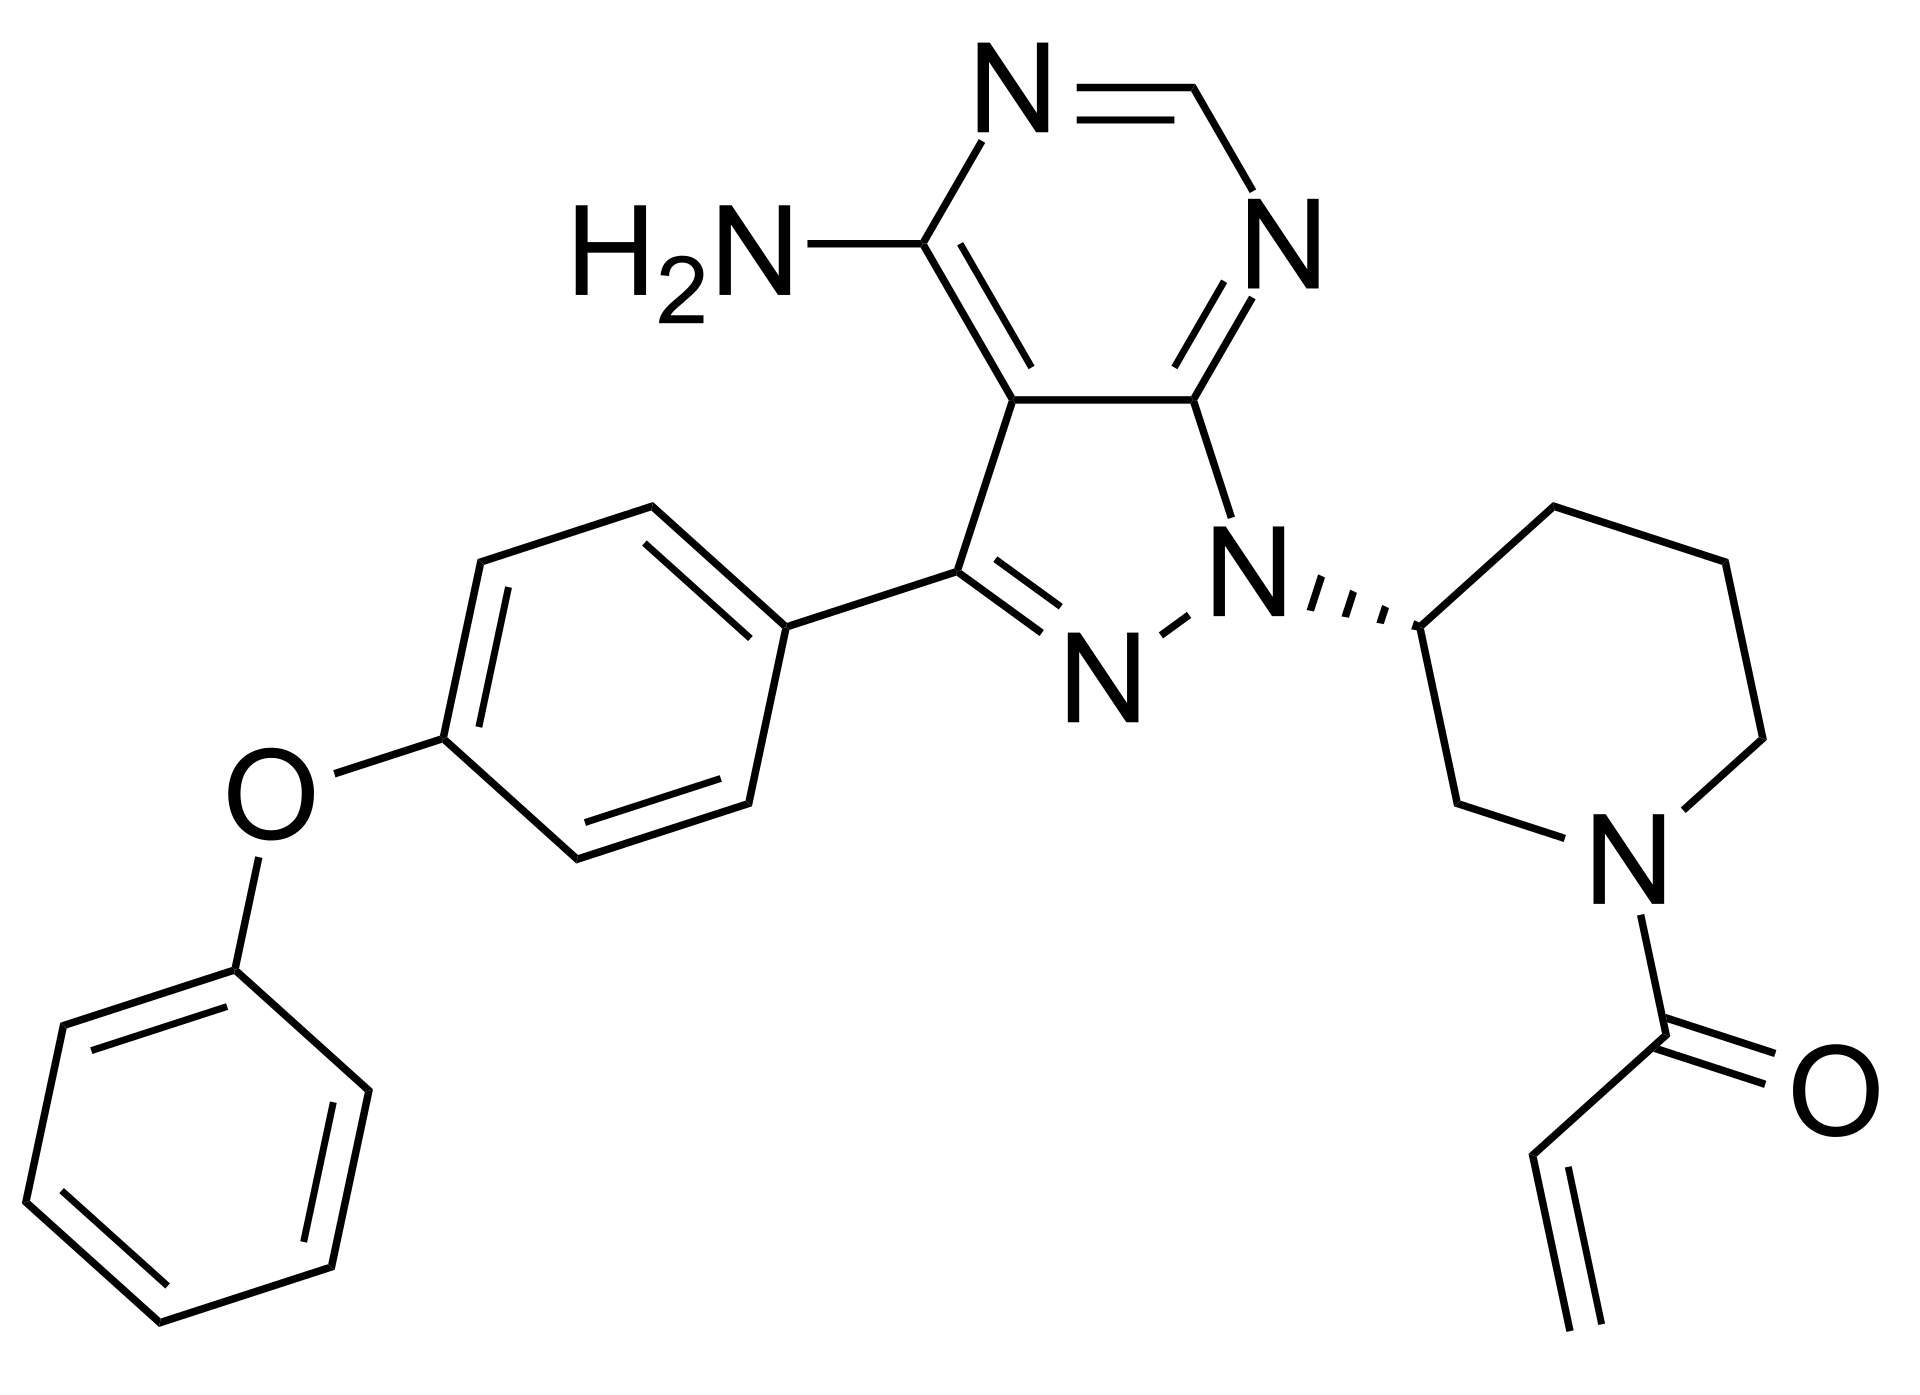
\includegraphics[scale=0.1]{Ibrutinib.png}
	\caption{Molecular structure of chemotherapeutic drug Ibrutinib}
	\label{fig:Ibr}
\end{figure}

%--------------------------
\subsection{Cytarabine (Cyt)}
Cytarabine (Cyt) is a medication used in treatment of leukemias and lymphomas. As it can be seen in Fig. \ref{fig:Cyt}, it is a nucleoside (pyrimidine analog) with arabinose sugar, also called arabinosylcytosine, and is an antimetabolite and antineoplastic.
The sugar moiety induces the rotation of Cyt within the DNA, blocking DNA replication during the S-phase of cellular replication. It also acts on DNA polymerase and its maximum effects are seen after the time equivalent to a full cell cycle (8-12 h). 
The drug is admnistered via intravenous infusion and it was shown that the dose-response relationship for Cyt has a plateau above a dose level of 1000 mg/$m^2$ (intermediate dose). The reported dosage for patients is a first cycle with 200 mg/$m^2$ of Cyt infused continuously for 24 hours, and a second cycle with 1000 mg/$m^2$ infused for three hours twice a day \cite{cyt-3}.
Cyt has two types of metabolites: 
\begin{itemize}
	\item \textbf{inactive metabolites}, from deamination as soon as the drug enters the plasma
	\item \textbf{active metabolites} (Cyt triphosphate, CytTP), after being transported into the cell, and after phosphorylation.
\end{itemize}
The active metabolites competitively inhibit DNA polymerase, they are incorporated into DNA where they act as chain terminator, leading to incomplete DNA replication and cell death.\\
CytTP has a saturation level, leading to accumulation of the metabolite in cells, a lower drug selectivity of cancer cells, and a higher degree of myelosuppression.\cite{cyt-1, cyt-2}
\begin{figure}[htbp!]
	\centering
	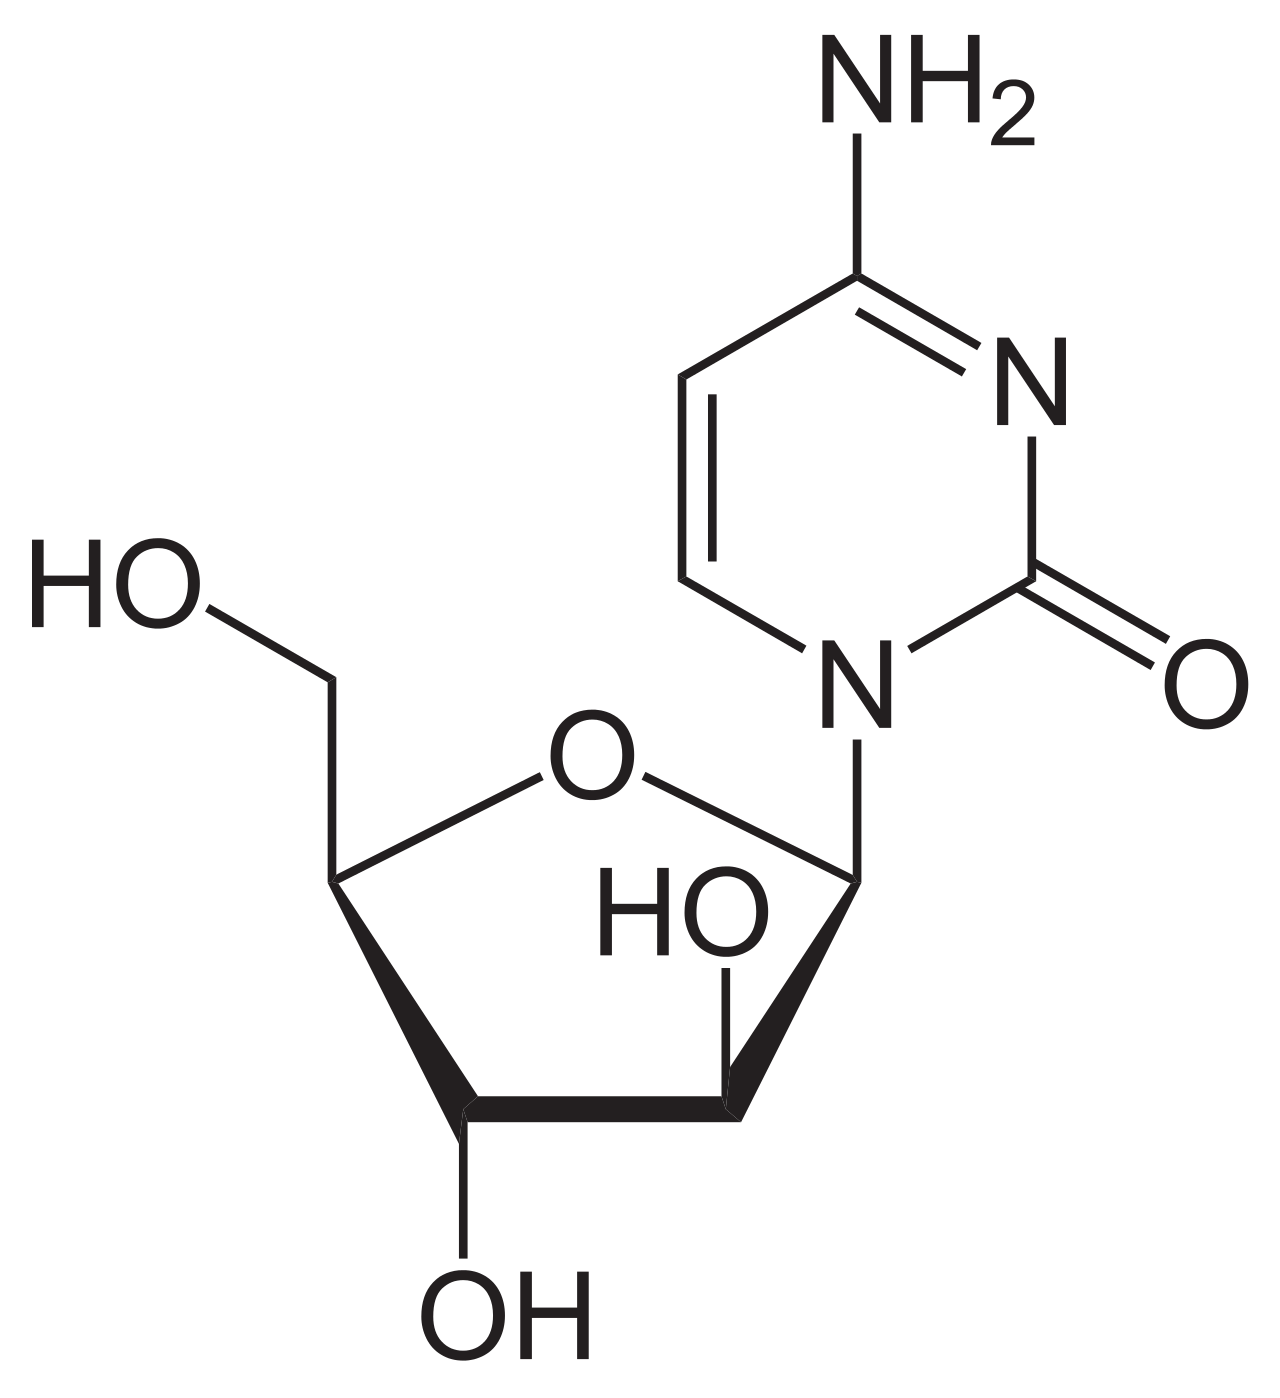
\includegraphics[scale=0.1]{Cytarabin.png}
	\caption{Molecular structure of chemotherapeutic drug Cytarabine}
	\label{fig:Cyt}
\end{figure}

